\chapter{Introduction}



%\marginpar[Margin note.]{Margin par.}



\section{Overview} 

The appearance of a 3D scene comprises the visual features that are defined by the interaction of light with materials, textures, and geometry, defining how we perceive objects in terms of colour, shading, and surface detail. Many factors, including lighting conditions, material properties, and environmental effects, affect appearance. For instance, lighting defines the illumination of objects with its type, location, intensity and colour, generating shadows, highlights, and the contrast. Materials describe the optical/reflectance properties, such as roughness, transparency, and base colour. Textures are the patterns that reveal details about a surface, such as bumpiness, or imperfections.The geometric detail and surface orientation affect the interaction of light with the object. Atmospheric conditions such as clouds, reflections, and global illumination also contribute to the appearance of a scene. Overall, appearance is the product of light-material interactions shaped by both surface detail, geometry and texture and environmental factors. 
 
Appearance manipulations refer to the edits of the aforementioned visual features, ranging from retouching intricate details to transforming entire scenes. Appearance manipulation techniques are instrumental in the success of multiple fields with real-world applications. In filmmaking, it helps create realistic special effects or offers subtle changes to lighting, costumes, and even an actor’s appearance during post-production. In social media and advertising, it allows users to benefit from filters, face-tuning, and other aesthetic tools. In augmented and virtual reality (AR/VR) platforms, it enables embodying human avatars that improve immersive realism, including changing hairstyles, outfits or body types. In fashion and e-commerce, users can faithfully shop clothes or accessories online through virtual try-ons. 

Even the fact that Richard Linklater had filmed the movie "Boyhood" (2014) over 12 years to capture the natural aging of the actors shows the necessity and importance of precise appearance manipulation techniques across disciplines. Therefore, this thesis is dedicated to tackle the challenging task of appearance manipulations with learning-based techniques with the hope that the proposed approaches can alleviate some of the difficulties that editors come across, such as accuracy, the scarcity of data, etc. This thesis investigates the three distinct perspectives of appearance (fine details, transient attributes, reflectance representations) and presents data-efficient machine learning approaches for accurate and visually-pleasing manipulations.

Earlier approaches to manipulate scene appearance involve traditional image processing/computer graphics techniques and extensive manual editing in dedicated software platforms, such as Photoshop, Lightroom, Blender or Unreal Engine. These traditional editing approaches require significant time and skill due to the complexity and scale of the transformations involved. On the other hand, recent advancements in machine learning techniques starting with convolutional neural networks and reaching the current state of generative models have paved the way for precise and natural-looking appearance transfers that maintain the photorealism of the rendered scene. For instance, we can now instruct programs to edit images in only a few seconds thanks to the developing field of generative AI. Furthermore, the deep learning models have allowed us to represent naturally continuous signals as continuous neural functions, which were before bounded to the discrete representations. 

Consequently, machine learning techniques have revolutionised appearance manipulation by generating high-quality, realistic renderings from data inputs. However, the main bottleneck in these approaches is the scarcity of the training data that can drastically reduce the performance of the ML models. For instance, the number of pixels that belong to details is significantly lower than those belonging to low-frequency components, or obtaining the real "summer" - "winter" image pair can require us to wait for months. Furthermore, capturing the real-world reflectance measurements of even relatively simple materials takes hours in a professional capture setup. For these reasons, this thesis specifically focuses on generalisable learning-based approaches that can manipulate appearance with data efficiency.

This dissertation studies appearance in a broader aspect, going beyond the 2D image representation of appearance and discussing its physics-based meaning in real-world 3D scenes. Therefore, I first begin with a background on rendering, providing essential information about the display of an image, 3D scene components, appearance representations and the rendering equation, bridging the appearance in a rendered image to reflectance and illumination in the 3D scene. I also provide details about the learning-based techniques I have deployed, starting with the basics of machine learning. Appearance in a 2D image involves low-level features that usually focus on pixel-level details with basic and simple visual elements and high-level features that represent more abstract, semantic information about the image. 

\subsection{One-shot detail retouching}
First, I introduce a machine learning framework designed to manipulate such low-level features, including edge, corners, and textures, learned from only one example \textit{before - after} pair. The framework can transfer the desired styles embodied in high-frequency components, while remaining generalisable across faces under different lighting conditions or with different skin tones. Working on the luminance channel, it utilises multi-spectral image decomposition, a Laplacian pyramid, to maintain control over high-frequency components at different scales. The weight assignment to image patches through a multilayer perceptron also allows similar patches to lie on the same transform space. This allows the model to be used as an edge-aware neural image processing filter, where the texture, such as skin, is smoothed out, and the edges are preserved. The transformations are defined as learnable matrices, where the matrices are multiplied with patches using the dot product. This mapping representation can be considered as a general form of convolution, in which the entries are learned during training. One-shot detail retouching can accurately transform the fine details into a desired form defined by the style in the example pair. Its applications can be most useful when details convey crucial information and consequently dominate the entire scene, such as in close-up shots (Figures \ref{fig:close-up1} and \ref{fig:close-up2}). 


%Appearance manipulation has become an indispensable tool in modern visual culture, driving innovation in entertainment, healthcare, and beyond. AI's involvement enhances the accuracy, scalability, and creativity of appearance modifications, pushing the boundaries of what is visually possible and enabling more seamless and engaging user experiences across industries.


%\subsection{One-shot Detail Retouching}

\begin{figure}[ht]
  \centering
  % \fbox{\rule{0pt}{2in} \rule{0.9\linewidth}{0pt}}

    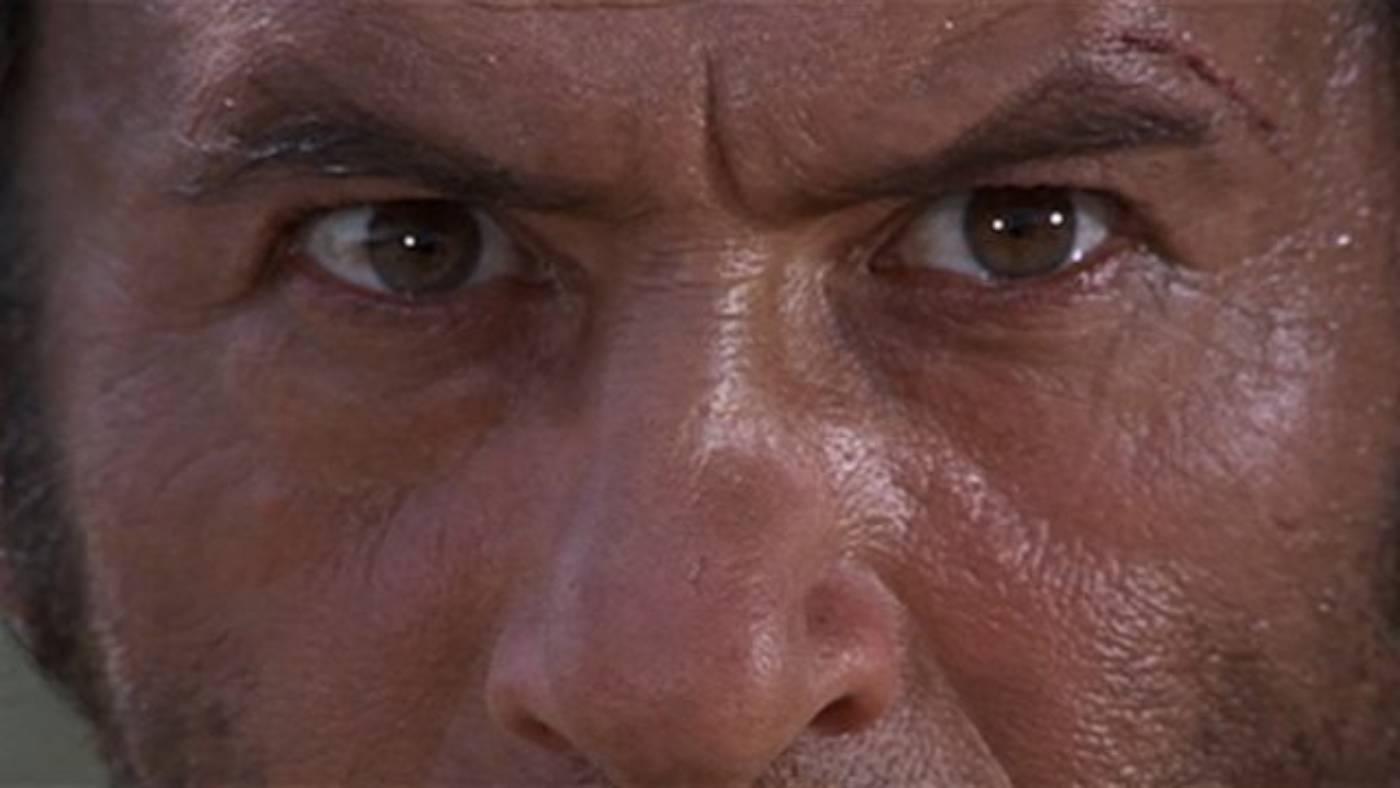
\includegraphics[width=\linewidth]{Images/A scene from ‘The Good, the Bad and the Ugly’ (1966). Image courtesy- Produzioni Europee Associati .jpg}

   \caption{A close-up scene from the movie ‘The Good, the Bad and the Ugly’ (1966). Details can convey valuable information about a scene, such as wrinkles hinting at the character's age in this shot. Image courtesy of [Produzioni Europee Associati].}
   \label{fig:close-up1}
\end{figure}


\begin{figure}%{r}{5cm}
  \centering
  % \fbox{\rule{0pt}{2in} \rule{0.9\linewidth}{0pt}}
   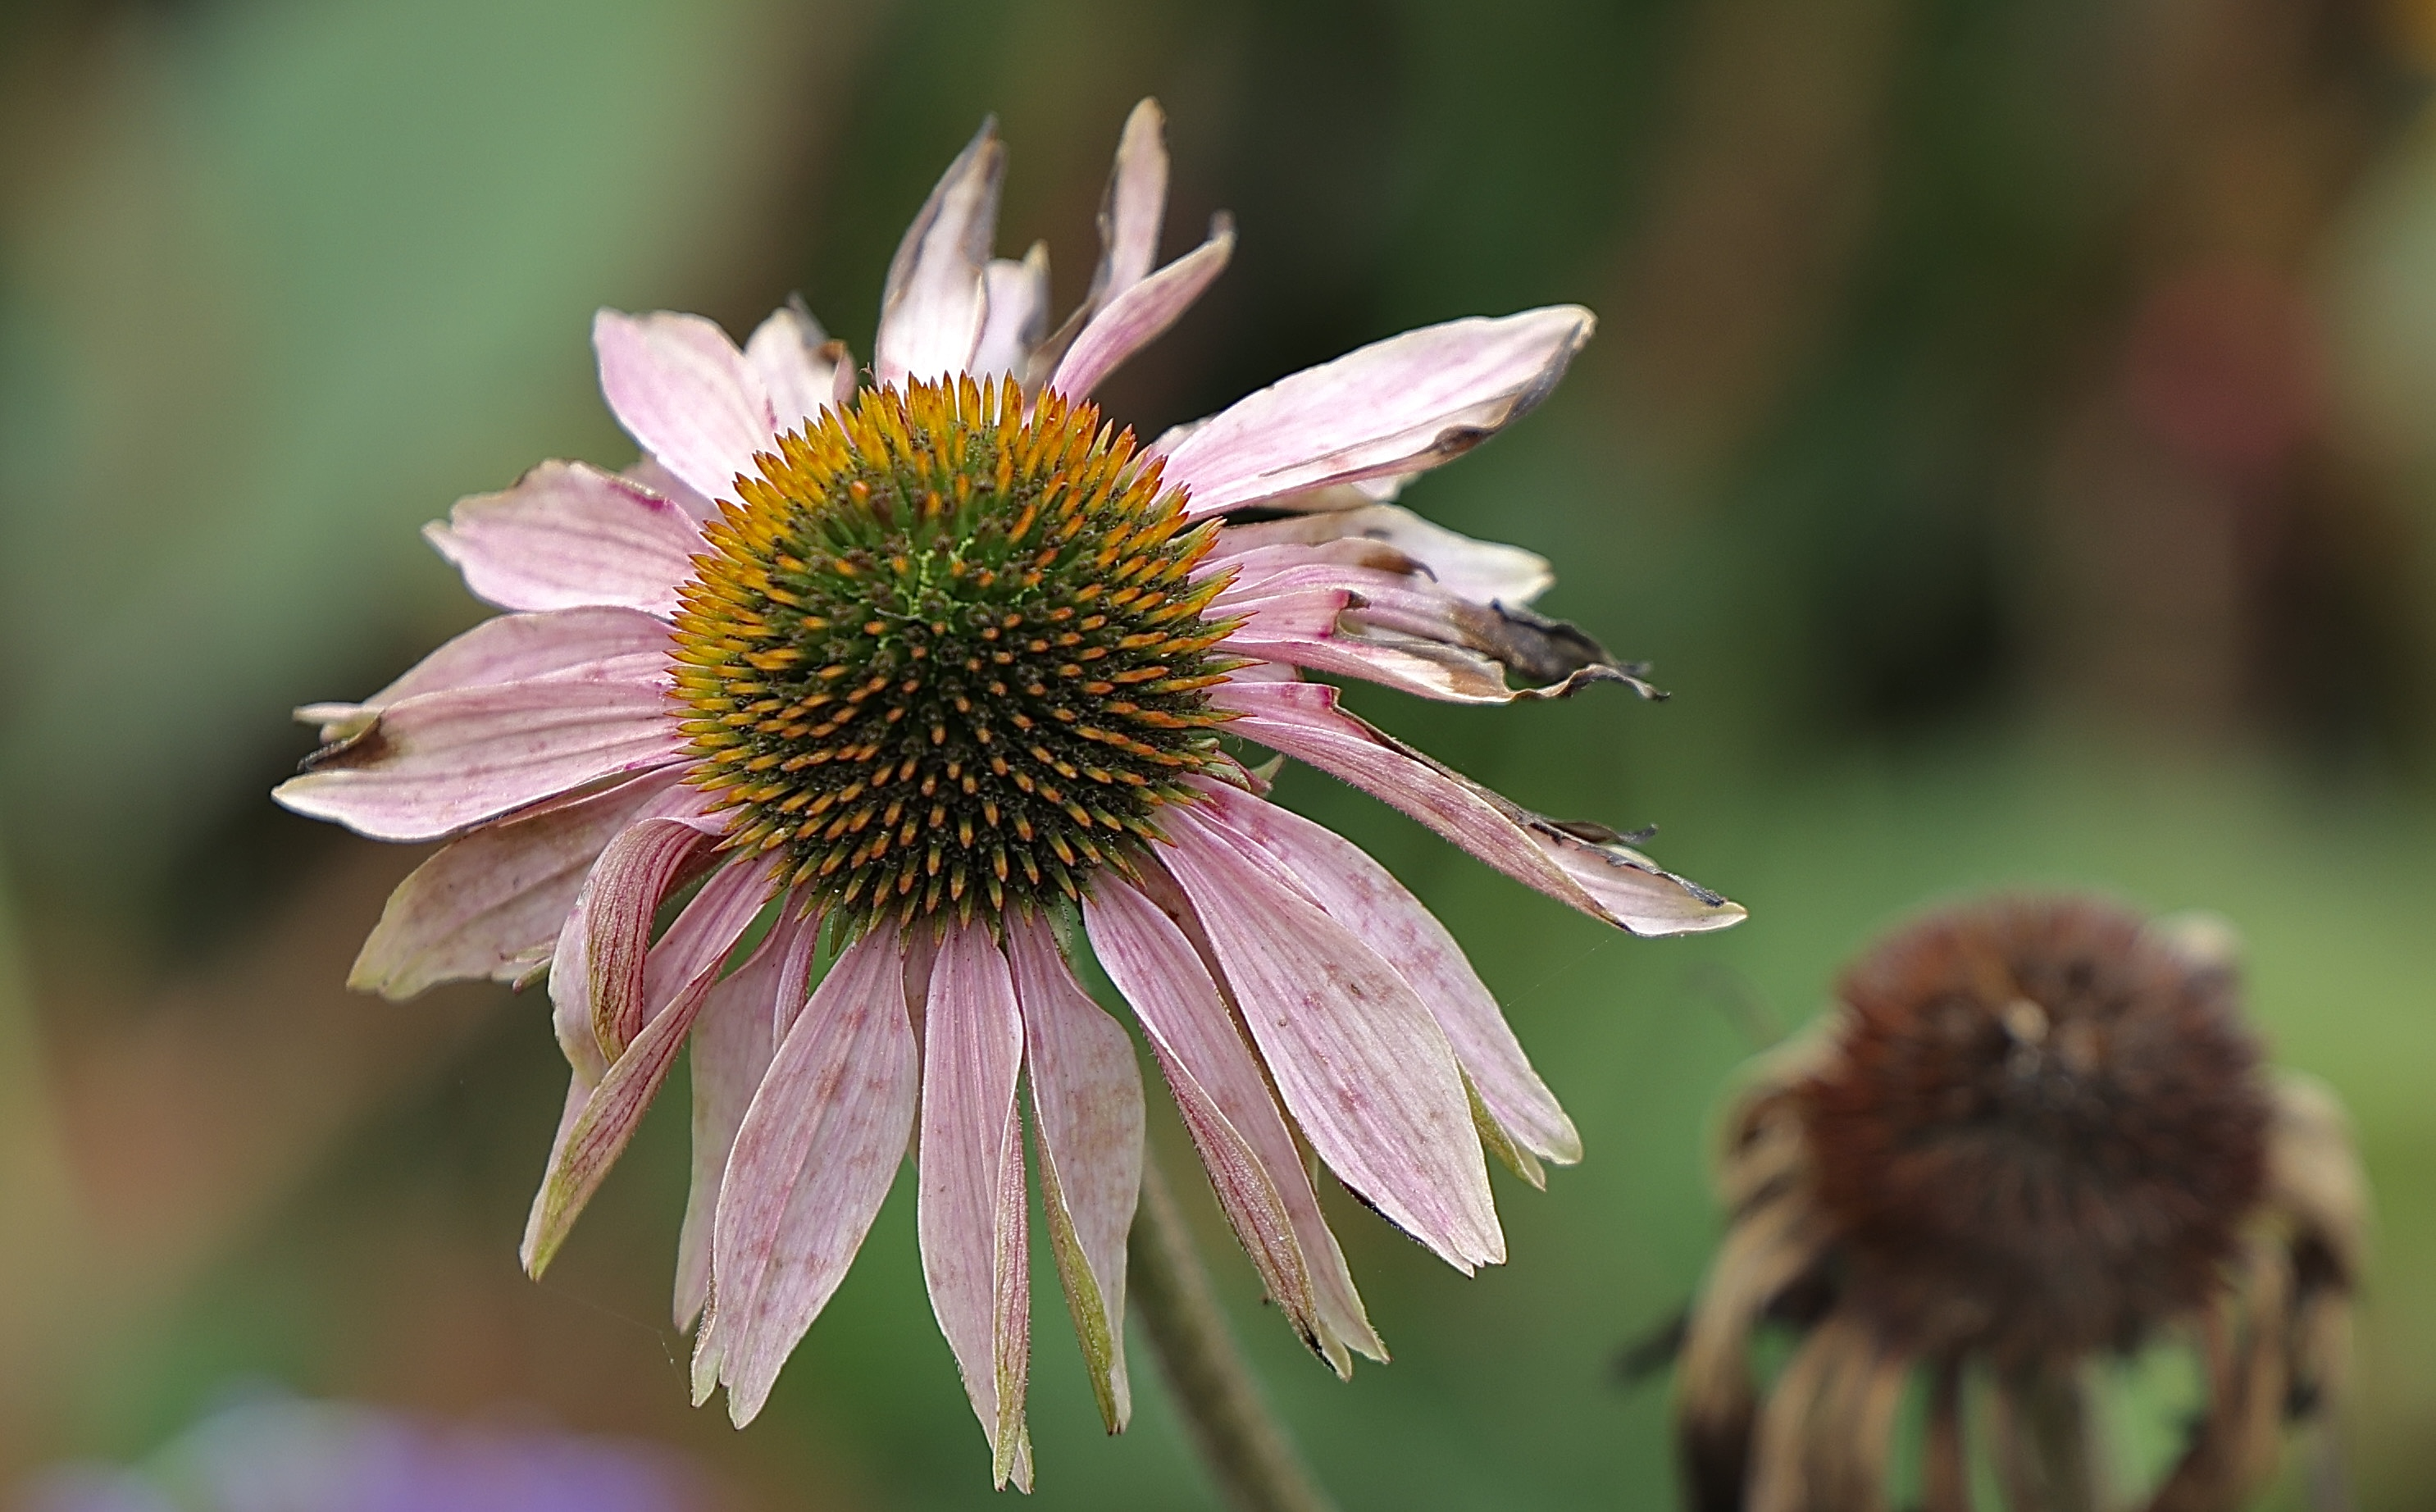
\includegraphics[width=\linewidth]{Images/flower-closeup.JPG}
   
   \caption{Another close-up shot example. In photography, captivating details contribute to aesthetics, highlighting the identity of the subject.}
   \label{fig:close-up2}
\end{figure}

%[Andrew Fusek Peters].

%\newpage
\subsection{Text-guided transient attribute transfer} 

\begin{figure}[ht]
  \centering
  % \fbox{\rule{0pt}{2in} \rule{0.9\linewidth}{0pt}}

    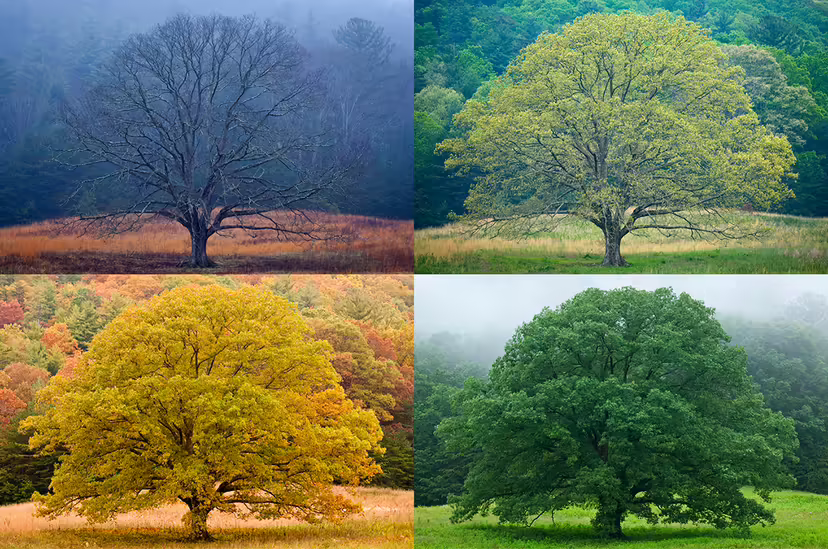
\includegraphics[width=\linewidth]{Images/seasonchanges.png}

   \caption{Seasonal transitions of a tree throughout the year. Image from [Michael Melford/Getty Images]}
   \label{fig:colour-approximate}
\end{figure}

Second, I explore the transitions between transient attributes, which cover manipulations on high-level features with global illumination changes, colour transfers, object addition/removal, and so on. Borrowing the pre-trained text-guided diffusion models, I investigate their tuning-free capacity for transferring transient attributes.
\subsection{Generalisable Neural BRDF Representation}
Lastly, I introduce HyperBRDF, a novel neural material appearance representation method that can generalise well to new materials, offering state-of-the-art results in sparse reconstruction and compression. HyperBRDF is the first of its kind, introducing a generalisable neural field for bidirectional reflectance distribution function (BRDF) representation. BRDF defines the ratio between the incident and outgoing light intensities for a specific material and can be used to compute the shading of materials in physics based rendering (PBR) pipelines. PBR characterises light-material interactions more accurately, hence offering realistic renderings that are comparable with photographs (Figure \ref{fig:brdf-intro}). BRDF modelling is of crucial importance to the computer graphics community studying material/appearance models. However, the current methods usually rely on analytic models that approximate the highly complex BRDFs with only a few parameters, reducing the quality of the photorealism in rendered scenes. Another approach would be to incorporate the real-world measurements into PBR pipelines, defining BRDF as the sample values for corresponding incoming/outgoing light directions. Although real-world measurements offer precise representations of the reflectance, capturing these samples is highly costly and time consuming, requiring professional capture systems with heavy manual workload. Therefore, I design and implement a neural network based BRDF model that can reconstruct new materials with only a sparse set of samples.I demonstrate several applications of HyperBRDF, namely sparse reconstruction, compression, and editing, with outstanding performance. 

\begin{figure}[ht]
  \centering
  % \fbox{\rule{0pt}{2in} \rule{0.9\linewidth}{0pt}}

    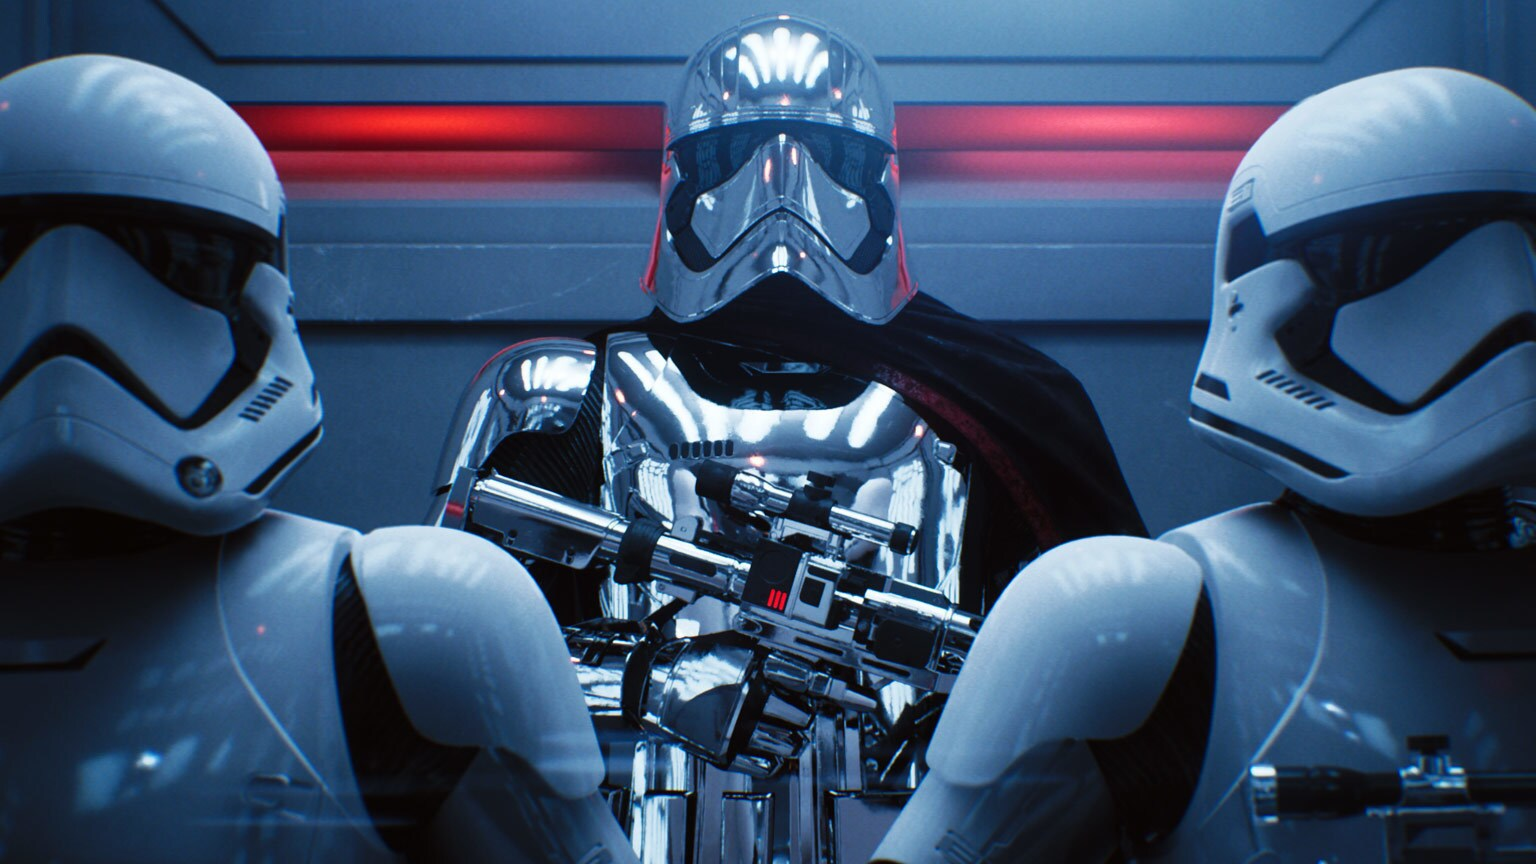
\includegraphics[width=\linewidth]{Images/StarWars-RayTracing.jpeg}

   \caption{Photorealistic rendering can be achieved through extensive ray tracing for which reflectance should be accurately measured and represented. Image from [Star Wars Real-Time Ray Tracing Demo by Epic Games, NVIDIA, and ILMxLAB].}
   \label{fig:brdf-intro}
\end{figure}



%\section{Contributions}
\section{Contributions and publications}

The following works are produced throughout my doctoral studies and contributed to main chapters of this dissertation:

\begin{itemize}

\item \textbf{Fazilet Gokbudak}, Alejandro Sztrajman, Chenliang Zhou,  Fangcheng Zhong, Rafal Mantiuk, and Cengiz Oztireli. Hypernetworks for Generalizable BRDF Representation. \textit{ECCV 2024}

\textit{Contribution:} Designed and implemented a novel neural BRDF representation model that can be used for sparse reconstruction, compression and editing, integrated into physically-based renderers.

\item \textbf{Fazilet Gokbudak} and Cengiz Oztireli. Text-guided Transient Attribute Transfer. \textit{Under review}.

\textit{Contribution:} Run an exploratory study on the ability of pre-trained diffusion models to capture complex transient attribute transfers.

\item \textbf{Fazilet Gokbudak} and Cengiz Oztireli. One-shot Detail Retouching with Patch Space Neural Transformation Blending. \textit{In Proceedings of the 20th ACM SIGGRAPH European Conference on Visual Media Production (CVMP '23)}, 2023. Association for Computing Machinery, New York, NY, USA, Article 2, 1–10. https://doi.org/10.1145/3626495.3626499

\textit{Contribution:} Designed and implemented a machine learning framework that can retouch details based on the style defined by a single example pair. 

\end{itemize}

The following works did not directly contribute to this dissertation; however, they helped me build skills and knowledge for the success of the main contributions:

\begin{itemize}

\item Madeleine Darbyshire, Shaun Coutts, Eleanor Hammond, \textbf{Fazilet Gokbudak}, Cengiz Oztireli, Petra Bosilj, Junfeng Gao, Elizabeth Sklar, and Simon Parsons. Multispectral Fine-Grained Classification of Blackgrass in Wheat and Barley Crops. \textit{Under Review}, 2024.

\item Chenliang Zhou, Alejandro Sztrajman, Rainer Gilles, and Fangcheng Zhong, \textbf{Fazilet Gokbudak}, Zhilin Guo, Weihao Xia, Rafal Mantiuk, and Cengiz Oztireli. Physically Based Neural Bidirectional Reflectance Distribution Function. \textit{Under Review}, 2024.

\end{itemize}